\documentclass[11pt]{article}   % tipo de documento e tamanho das letras

% os seguintes pacotes estendem a funcionalidade básica:
\usepackage[a4paper, total={16cm, 24cm}]{geometry} % tamanho da pagina e do texto
\usepackage[portuguese]{babel}  % traduz para portugues
\usepackage[utf8]{inputenc}
\usepackage{graphicx}           % graficos
\usepackage{amsmath}            % matematica
\usepackage{tikz}               % diagramas
    \usetikzlibrary{shadows}
\usepackage{booktabs}           % tabelas com  melhor aspecto
\usepackage[colorlinks=true]{hyperref}           % links para partes do documento ou para a web
\usepackage{listings}           % incluir codigo
    \renewcommand\lstlistingname{Listagem}  % Listing em portugues
    \lstset{numbers=left, numberstyle=\tiny, numbersep=5pt, basicstyle=\footnotesize\ttfamily, frame=tb,rulesepcolor=\color{gray}, breaklines=true}
\usepackage{blindtext}

% -------------------------------------------------------------------------------------------
\title
{
    
\includegraphics[width=0.3\textwidth]{images/logo_universidade.png}
    \\[0.1cm]
    \textbf{Gerador de Árvores de Decisão} \\
    Aprendizagem Automática
}

\author
{
    \textbf{Professores:} Teresa Gonçalves \\ Luís Rato \\
    \textbf{Realizado por:} Miguel de Carvalho (43108) \\ João Pereira (42864) 
}
\date{\today}

% -------------------------------------------------------------------------------------------
%                                Body                                                       %
% -------------------------------------------------------------------------------------------

\begin{document}
\maketitle

% -------------------------------------------------------------------------------------------
\section{Introdução} 

\hspace{0,5cm}Neste trabalho foi solicitado a realização de um programa que simule a criação de \textbf{Árvores de Decisão} com \textbf{pruning}, 
representado na figura abaixo. \par
\begin{figure}[h!]
    \begin{center}
	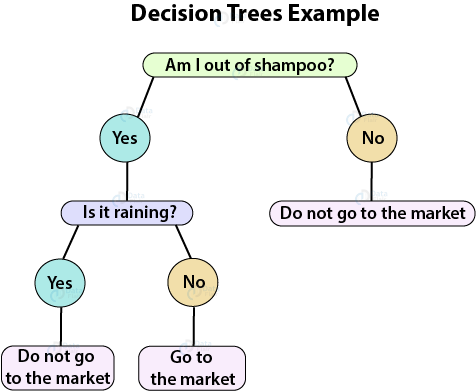
\includegraphics[width=0.5\textwidth]{images/tree-example.png}
        \caption{Exemplo de uma Árvore de Decisão}
    \end{center}
\end{figure}
A \textbf{Árvore de Decisão} é uma forma expressiva e fácil de perceber como será feita a decisão para os dados em questão.


É constituída por:
\begin{itemize}
    \item \textbf{Nós (Nodes)} são as perguntas feitas para ser tomada uma decisão, por conseguinte a decisão irá escolher por qual \textbf{ramo} vai passar;
    \item \textbf{Ramos (Branchs)} são as decisões que são tomadas, que vão levar a outro \textbf{nó} ou mesmo a uma \textbf{folha};
    \item \textbf{Folhas (Leafs)} é a \textbf{classe} (resposta final) que corresponde à(s) decisão(ões).
\end{itemize}
\begin{figure}[h!]
    \begin{center}
	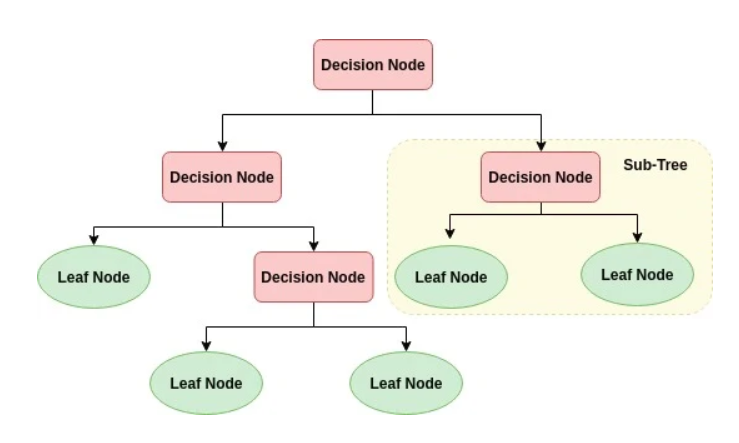
\includegraphics[width=0.5\textwidth]{images/tree-structure.png}
        \caption{Estrutura de uma Árvore de Decisão}
    \end{center}
\end{figure}


Existem vários \textbf{critérios} para realizar a decisão de qual deverá ser o \textbf{nó} escolhido, ou seja,
qual deverá ser a melhor questão a ser feita em cada instante. \par
Neste trabalho serão utilizados o seguintes critérios \textbf{Entropia}, \textbf{Gini} e o \textbf{Erro}:
\begin{itemize}
    \item A \textbf{Entropia} é a informação esperada em bits;
    \item O \textbf{Gini} é o erro esperado se etiquetar as folhas aleatoriamente; 
    \item O \textbf{Erro} é também conhecido como razão do erro.
\end{itemize}

% -------------------------------------------------------------------------------------------
\section{Implementação}
\hspace{0,5cm}Inicialmente começámos por analisar os dados que nos foram fornecidos e tentámos criar
a \textbf{Árvore de Decisão} com os dados mais pequenos, realizando todos os cálculos. Para podermos 
ter uma ideia do que o nosso programa iria ter que realizar.

Por conseguinte começámos por tentar automatizar a leitura e os cálculos todos necessários para que funcionasse
com o critério \textbf{Entropia}.

Após termos conseguido realizar tudo na prática para os dados do \textbf{Weather} e com o critério
\textbf{Entropia}, tentámos com o resto dos dados que foram disponibilizado pelos professores e 
fizémos as devidas correções para que funcionasse com todo o tipo de dados.

De seguida, começámos por implementar os dois restantes critérios, o \textbf{Gini} e o \textbf{Erro}.

Por último, testámos novamente com todos os dados e fizemos as devidas correções.
% -------------------------------------------------------------------------------------------
\section{Funções}
\begin{itemize}
    \item Classe \verb|node|: classe que representa cada \textbf{nó} ou \textbf{folha} da \textbf{Árvore de Decisão}.
    \begin{itemize}
        \item \verb|is_leaf|: função que retorna \verb|true| se o \textbf{nó} não tiver \textbf{folhas}(filhos);
        \item \verb|set/get_Data|: função que define o conteúdo do \textbf{nó};
        \item \verb|set/get_Sons|: função que lista de referencias dos \textbf{nós} filhos;
        \item \verb|sons_order|: função que caso o \textbf{nó} seja considerado um \textbf{nó} esta variável consiste numa lista que possui a ordem de "distribuição" dos valores de um dado atributo.
    \end{itemize}
    \item Classe \verb|myDecisionTreeREPrune|: classe que representa a \textbf{Árvora de Decisão}
    \begin{itemize}
        \item \verb|fit|: função que constrói a \textbf{Árvora de Decisão};
        \item \verb|homogeneous|: função que recebe os valores de classe dos objetos de teste
        e averigua se os dados são homogéneos, ou seja, todos os objetos possuem a mesma classificação.
        Caso possuam, é feito o \verb|return| do valor da classe comum a todos objetos e a \textbf{árvore} consiste numa única \textbf{folha} 
        (com o valor dessa classe)
        \item \verb|grow_tree|: função que constrói a \textbf{árvore} com o auxilio das seguintes funções:
        \begin{itemize}
            \item \verb|globalTotalValues|: função que retorna num array quantas vezes aparece cada class
            \item \verb|entropyCalc|: função que recebe como argumento o numero de vezes que cada classe aparece e calcula a \textbf{entropia};
            \item \verb|giniCalc|: função que recebe como argumento o número de vezes que cada classe aparece e calcula o \textbf{gini};
            \item \verb|errorCalc|: função que recebe como argumento o numero de vezes que cada classe aparece e calcula o \textbf{erro};
            \item \verb|chooseNode|: função que recebe a lista de \verb|attributes| e calcula o ganho de cada e \verb|retorna| o atributo com maior ganho,
            o atributo principal;
            \item \verb|checkLeaf|: função que verifica se os valores de um determinado atributo podem determinar a classe de um objeto \textbf{(folha)},
            a função retorna uma lista dos "valores \textbf{folha}" e uma lista com as respetivas classes;
            \item \verb|isLeaf|: função que verifica se um atributo é uma \textbf{folha}, ou seja, só já tem uma classe;
            \item \verb|valuesNotToLeafs|: função que verifica se um determinado valor do atributo não é uma \textbf{folha};
            \item \verb|setSons|: função que define os filhos do \textbf{nó}. Os filhos podem ser \textbf{folhas} ou podem ser \textbf{ramos};
            \item \verb|removeAttribute|: função que remove um atributo especifico de uma lista de atributos retorna a lista sem o atributo e 
            a posição onde este se encontrava;
            \item \verb|appendAttribute|: função que adiciona um atributo especifico a uma lista de atributos retorna a lista com o atributo 
            na posição especificada;
            \item \verb|update_data|: função que \textbf{restringe} a data do conjunto de treino, retorna a data resultante dessa restrição 
            e as diferenças entre o original e a data resultante;
            \item \verb|applySaves|: função que \textbf{reverte} as alterações aplicadas no conjunto de teste. Para isso é necessário voltar 
            a colocar o valor removido no local correto e de seguida colocar todas as \textbf{linhas} nas posições corretas;
            \item \verb|getValues|: função que retorna um array com os valores de um dado atributo;
            \item \verb|valueCount|: função que conta o número de classes correspondentes a um value de um dado atributo;
            \item \verb|calculateGain|: função que retorna o ganho de uma classe;
            \item \verb|entropyRootValues|: função que devolve a entropia de cada value do Atributo Principal \textbf{(nó principal)}.
        \end{itemize}
        \item \verb|score|: função que utiliza um conjunto de dados de teste para avaliar a \textbf{árvore de decisão} construida;
        \begin{itemize}
            \item \verb|iterate_for|: função que recebe um \textbf{objeto} do conjunto de teste e faz uma \textbf{iteração} pela \textbf{árvore de decisão} com o objetivo de obter 
            uma classificação. De seguida, essa decisão vai ser comparada com o valor esperado do objeto, se ambos forem idênticos, dá return de um \textbf{"hit"},
            caso contrário, dá return de um \textbf{"miss"}.
        \end{itemize}
    \end{itemize}
\end{itemize}
% -------------------------------------------------------------------------------------------
\section{Execução}
\hspace{0,5cm}Para executar o \textbf{gerador de Árvores de Decisão} o utilizador deverá passar como argumento o ficheiro de \textbf{input}.
Argumentos do Programa:
\begin{itemize}
    \item Localização do ficheiro \verb|"-f ficheiro.csv"| - argumento necessário, com a localização do ficheiro com os dados;
    \item Escolha do critério \verb|"-c critério"| - por default o critério é \textbf{entropy}. Pode ser: \textbf{entropy}, \textbf{gini} ou \textbf{error};
    \item Ligar/Desligar \textbf{pruning} \verb|"-p"| - por default o \textbf{pruning} está desligado.
\end{itemize}
\par Exemplos:
\begin{itemize}
    \item \verb|python myDecisionTreeREPrune.py -f dados/vote.csv| irá executar o \textbf{gerador de Árvores de Decisão} utilizando o critério \textbf{Entropy} com os dados do \verb|vote.csv| e \textbf{sem Pruning};
    \item \verb|python myDecisionTreeREPrune.py -f dados/soybean.csv -c gini| irá executar o \textbf{gerador de Árvores de Decisão} utilizando o critério \textbf{Gini} com os dados do \verb|soybean.csv| e \textbf{sem Pruning};
    \item \verb|python myDecisionTreeREPrune.py -f dados/weather.nominal.csv -c error| irá executar o \textbf{gerador de Árvores de Decisão} utilizando o critério \textbf{Error} com os dados do \verb|weather.nominal.csv| e \textbf{sem Pruning};
    \item \verb|python myDecisionTreeREPrune.py -f dados/vote.csv -c gini -p| irá executar o \textbf{gerador de Árvores de Decisão} utilizando o critério \textbf{Gini} com os dados do \verb|vote.csv| e \textbf{com Pruning};
\end{itemize}
% -------------------------------------------------------------------------------------------
\section{Análise de Resultados}
\subsection{weather.nominal.csv}
    
No \verb|weather.nominal.csv|, a \textbf{árvore de decisão} foi bem construida com as todas funções de impureza e o score apresenta uma alta taxa de sucesso.

\subsection{contact-lenses.csv}

No \verb|contact-lenses.csv|, a a \textbf{árvore de decisão} foi bem construida com as todas funções de impureza e o score apresenta uma taxa alta de sucesso.

\subsection{vote.csv}

No \verb|vote.csv|, o score apresenta uma taxa média de sucesso, deduzimos que se deve ao facto das funções \verb|update_data| e \verb|applySaves| durante o 
crescimento recursivo da \textbf{árvore} corromperem os dados do conjunto de treino.
O \textbf{programa} demonstra um grande tempo de execução com os dados deste ficheiro, o que demonstra que deverá ser um \textbf{problema de otimização}.

\subsection{soybean.csv}

No \verb|soybean.csv|, os \textbf{problemas de otimização} não permitem que o programa terminem.
% -------------------------------------------------------------------------------------------
\section{Conclusão} % Conclusão
\hspace{0,5cm}Em suma, com a realização deste trabalho "Gerador de Árvores de Decisão" ficámos muito mais esclarecido sobre como é
feito o processo para gerar um \textbf{Árvore de Decisão}. \par
Processo este que pode ser feito com diferentes \textbf{critérios} que vão influenciar o resultado final.

As principais dificuldades foram o facto de o trabalho ter sido proposto com uma linguagem de programação no qual não nos
sentíamos à vontade, o \textbf{Python}.
Além disso foi assegurar que as funções \verb|update_data| e \verb|applySaves| cumprissem bem a sua funcionalidade, o que infelizmente não
foi possível.
% -------------------------------------------------------------------------------------------
\end{document}
